\shorthandoff{"}
\chapter{Stand der Forschung (4 Seiten)}
\label{ch:standDerForschung}
Sämtliche untersuchten Arbeiten setzen voraus, dass die Fähigkeiten der Mitarbeiter und die benötigten Kompetenzen der Stellen in einer strukturierten Form vorliegen. Die gängigste Darstellungsform ist dabei eine Matrix, welche über boolsche Werte oder Bewertungsskalen die Ausprägungen der Fähigkeiten jedes Mitarbeiters erfasst \cite[S. 11f.]{recommenderSystems:2016}. Ein Beispiel für eine solche Matrix ist in Abbildung \ref{fig:standDerForschung:abb1} dargestellt.\\
\begin{figure}[h]
	\centering
	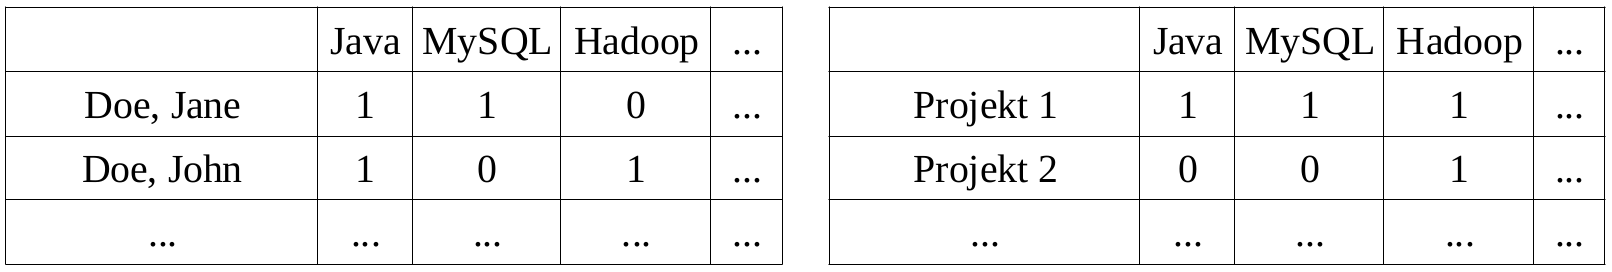
\includegraphics[width=1\textwidth]{gfx/Projektmatrix.png}
	\caption{Beispiel für eine Matrixdarstellung}
	\label{fig:standDerForschung:abb1}
\end{figure}
\\
Sämtliche Wissenschaftler in der Literatur sind sich einig, dass für die Empfehlung geeigneter Kandidaten für eine Stelle ein einfacher, boolscher Abgleich zwischen gesuchten und vorhandenen Fähigkeiten in den Matrizen eine unzureichende Lösung ist \cite[S. 2]{prospect:2010}\cite[S. 1]{enhancingERecruitment:2012}\cite[S. 1]{faerber:2003}. So kritisieren beispielsweise Gertner et al., dass bei einem solchen Ansatz Synonyme und ähnliche Fähigkeit nicht in die Suche einbezogen werden \cite[S. 1f.]{mitre:2014}.\\
Aus diesen Gründen ist der gängige Ansatz in der Literatur, ein Empfehlungssystem zu implementieren. Im englischsprachigen Raum ist der Begriff unter der Bezeichnung "Recommender System" verbreitet und wurde im Jahr 1997 von Paul Resnick und Hal R. Varian geprägt \cite{resnick:1997}. Ein Empfehlungssystem hat das Ziel, für eine große Menge von Elementen vorherzusagen, wie gut diese für die Anfrage eines Nutzers geeignet sind und sie in eine entsprechende Reihenfolge zu bringen \cite[S. 3]{recommenderSystems:2016}.



- \cite{mitre:2014}: Problem: Synonyme und ähnliche Begriffe werden nur schwer erkannt \\
- \cite{enhancingERecruitment:2012}: Quelle 12 zeigt, dass Boolsches Matching nicht gut funktioniert und viele Kandidaten nicht rekrutiert wurden / Quelle 6 zeigt, dass Keyword-Matching unzureichend ist \\
- "Es ist klar, dass Keyword-basiertes Skill-Matching nicht ausreicht", \cite{prospect:2010} \\
- \cite{aCollaborativeRecommenderSystemCourses:2016}: Erfolgreichste Plattformen, auf denen RS eingesetzt werden: Amazon und Netflix --> System von Netflix: Cine-Match \\
- \cite{malinowski:2008}: For this,recommender systems, used especially in E-commerceapplications to assist customers in finding the products orservices that match with their individual preferences,have recently received broad attention \\
- \cite{comibingCareer:2013}: RS sollen für Nutzer die Notwendigkeit der manuellen Suche entfernen \\
- \cite{malinowski:2006}: Quelle 23 etablierten den Begriff RS im Jahr 1997 \\
- \cite[S. 1]{enhancingERecruitment:2012} zeigt, dass RS erfolgreich z.B. Bei Amazon und Netflix eingesetzt werden \\

\section{Wissensbasierte Ansätze}
\label{ch:standDerForschung:wissensbasierteAnsaetze}
- \cite{malinowski:2008} SAP R/3 Human Resources und SP-Expert von Astrum speichern Skills in DB und versuchen anschließend ein Match zu finden / Schlüsselwort-Abgleich ist unzureichend / Quelle 4: Keyword-Abgleich in Marine-Schule / Quelle 9: Schlüsselwort-Abgleich ist unzureichend, da zu hohe Komplexität im Auswahlprozess\\
- \cite{malinowski:2006}: (Zum damaligen Zeitpunkt) verbreiteter Ansatz: Skill-Match über Keywords mit darunterliegender Ontologie --> Verwendet z.B. von SAP R/3 Human Resources und SP-Expert von Astrum --> Diese Ansätze reichen nicht aus \\
- \cite{semanticMatchmaking:2009}: Quelle Lau und Sure 2002 wendeten Ontogoloe-Basiertes Skill-Matching an / Colucci et al 2003: Wendeten Ontologie an / Bizer et al 2005 und Mochol et al 2007 suchten Ähnlichkeiten in Ontologien / Bianchiniet et al 2007 stellen fest, dass Ontologien sehr hohe Genauigkeit (Precision und Recall) bieten, dafür aber wenig flexibel sind (Flexibel definiert als: Fähigkeit Ergebnisse zu finden, wenn kein exaktes Match existiert) --> Flexibilität heute aber wichtig, da es nur selten der Fall ist, dass ein Individuum alle Skills hat / Wil Onotologie-Matching mit Flexibilität: Erstellt eine DL (Description Logic) mit OWL-DL --> Skills werden sehr feingranular hinterlegt, wobei zum Skill Leistungsnachweise hinterlegt werden müssen --> Passende Nutzer werden über Logik-Matching geladen --> Anschließende Sorteriung über Ähnlichkeitsmaße --> Ergebnis: Hohe Precision und Recall und gleichzeitig flexibel --> Anmerkung von mir: Sehr kompliziert zu pflegen / Unterscheidung Must-Have und Nice-To-Have /  \\
- \cite{exploringJobRecommentations:2019}: Quelle 29 entwickelt ein KB-Vorschlagssystem (sollte ich mir ansehen)\\
- \cite{aCombinedRepresentation:2018}: O*NET Onotologie des US Ministeriums für Arbeit nicht geeignet, da Entwicklung zu schnell, um Skills aktuell zu halten\\
- Gängige Meinung ist daher, dass CF bzw. CB verwendet werden sollten \\
- \cite{jobRecommenderSystemsASurvey:2012}: Proactive (Quelle 16) nutzt Ontologie

\section{Ansätze mit kollaborativem Filtern und inhaltsbasiertem Filtern}
\label{ch:standDerForschung:cfundcb}
- \cite{weightedSimilarity:2015}: Ähnlichkeitsbasierte Algorithmen werden auch als Memory-Basierte CF-Techniken bezeichnet\\
- Mitre führte Ähnlichkeitssuche über Jaccard-Koeffizienten durch \cite{mitre:2014} \\
- \cite{buildingVectorRepresentations:2020}: Verbindet Kandidaten mit Projekten, die relevant für die Skills sind / Projekt und Kandidat liegen in textueller Beschreibung vor --> Skill-Extraktion --> Darstellung als Vektor --> Ähnlichkeiten über Jaccard bestimmt \\
- \cite{malinowski:2008} Färber et al entwickelten ein System, welches CV-Daten von Bewerbern mit vergangenen Entscheidungen von HR trainiert wurden \\
- \cite{comibingCareer:2013}: Aktuelle Systeme suchen nach Ähnlichkeiten in Schlüsselwörtern --> Problem: Keine einheitliche Terminologie in Lebensläufen und Ausschreibungen --> Wenn Schlüsselwörter nicht gleich sind, gibt es kein Match über Ähnlichkeitsmaße / Auch ein Problem: Schlüsselwörter können falsch interpretiert werden, wenn Kontext nicht bekannt ist, z.B. "Networking"\\
- \cite{jobMatcher:2020}: Job Matching über CF --> Verwendet wegen Netflix, Amazon --> Sind die erfolgreichsten RS-Methoden (hier meine Kritik) / 68 Teilnehmer / Gibt an, bessere Ergebnisse als LinkedIn zu erzielen \\
- \cite{enhancingERecruitment:2012}: CB-System, wobei unterschiedliche Ähnlichkeitsmaße miteinander verglichen werden / Klappt sehr gut --> Hat aber auch nur 5 Kandidaten (?) mit sehr klar getrennten Skills \\
- \cite{dynamicUserProfile:2013}: Sucht passende Jobs über Ähnlichkeiten zu anderen Nutzern \\
- \cite{weightedSimilarity:2015}: Allgemein: Vorteil modellbasiert: Weniger Berechnungszeit; Vorteil Memorybasiert: Es müssen weniger Parameter abgestimmt werden \\
- \cite{personJobFit:2018}: Entwickeln modellbasierten Ansatz mit Convolutional Neural Networks (CNN), um Talent-Qualifikationen auf Job-Anforderungen zu matchen / CNN lernt aus historischen Job-Bewerbungen passende Person-Job-Fits zu erkennen / CNN kann auch erkennen, welche spezifischen Anforderungs-Items ein Kandidat erfüllt / Messen Distanz

\section{Grenzen einfacher Verfahren}
\label{ch:standDerForschung:grenzen}
- Long-Tail \cite{mitre:2014} und Data Sparsity \\
- \cite{malinowski:2008}: Quelle 3: Nachteil an CB --> Funktioniert nicht gut bei sehr diversen Features und es kann zu Überspezifizierung kommmen / Quelle 67: Nachteile bei CF: Data Sparsity --> Cold Start Problem / Quellen 18, 56, 66 sagen deshalb: Hybride Methoden
- Cold-Start \\
- \cite{weightedSimilarity:2015}: Traditionelle ÄHnlichkeitsmaße wie PCC, COS und MSD funktionieren nicht gut, wenn man zu wenige Bewertungen hat, zwischen denen man die Ähnlichkeit zwischen Nutzern berechnen kann (Cold-Start) --> Autor macht Vorschläge wie man damit umgehen kann / Sparse-Data-Problem wird mit hybriden Ansätzen angegangen / Gibt auch Graphenbasierte Ansätze

\section{Umgang mit dem Sparse Data-Problem}
\label{ch:standDerForschung:sparseData}
- Mitre kombiniert CB mit Interaktionen des Nutzers --> Ähnlichkeitssuche in einem Graphen und Anwendung des PageRank-Algorithmus \cite{mitre:2014} \\
- \cite{enhancingERecruitment:2012}: Quelle 9 unterscheidet zwischen Must-Have und Nice-To-Have \\
- \cite{buildingVectorRepresentations:2020}: Quelle 11 erstellt ein Job-RS und aktualisiert die Nutzerprofie dynamisch \\
- \cite{weightedSimilarity:2015}: Führt neue Gewichtungsschemata ein, die es erlaubt, neue Features zu berücksichtigen, um Ähnlichkeiten zwischen Nutzern zu finden --> Dabei werden symmetrische Schemata in asymetrische Schemata überführt, wobei die Bewerungen von Nutzern für nicht-gemeinsame Items berücksichtigt werden / Leisten zwei Beiträge: 1. Schlagen neuen Faktor vor, der zwischen dem Einfluss von Nutzern auf seine Nachbarn und umgekehrt erhält; 2. Analyse von Ähnlichkeiten zwischen Bewertungen unabhängig von Items

\section{Hybride Verfahren}
\label{ch:standDerForschung:hybrideVerfahren}
- \cite{hybridImmunizing:2017}: Verbessern Qualität der Empfehlung \\
- \cite{dynamicUserProfile:2013}: Quellen 14 und 15: Hybride Ansätze bringen akkuratere Ergebnisse \\
- \cite{combiningCbAndCFCostSensitiveApproach:2017}: Kombiniert CB und Cf --> Quelle 5 sagt, dass hybride Verfahren bessere Ergebnisse liefert / Frage: Passt Nutzer zum Job? / Quelle 32: Hybrides System auf Basis vergangener Bewerbungen / Quelle 33: Erstellte Graph mit CB und Ähnlichkeitsbestimmung zw. Profilen / Quelle 35 ist ähnlich zu dieser Arbeit, verwendet aber Markow-Logik-Netzwerke für hybriden Ansatz --> Diese Arbeit zeigt, dass dieser Ansatz nicht gut funktioniert \\

\section{Bilaterale Verfahren}
\label{ch:standDerForschung:bilateraleVerfahren}
- \cite{malinowski:2008}: "Existing systems only consider whether a person has the requiredtechnical skills and abilities for a job." / Quelle 2: Existing approaches usually consider only unary attri-butes that are tied directly to an individual (e.g.educational data) and–based on them–assess theaptitude of a candidate in relation to the job requirements\\
- \cite{jobRecommenderSystemsASurvey:2012}: Quelle 15: Bilaterales Sytstem / Quelle: Piazzato baut Reciporal Reommender für Jobs / Zu Reciprocal wenig Literatur\\
- \cite{hybridImmunizing:2017}: Entwickeln hybrides System unter Beachtung des bilateralen Systems \\
- \cite{malinowski:2006}: Theorie zeigt, dass für ein gutes Match eine bilaterale Beziehung bestehen muss\\
- \cite{malinowski:2008} orientiert sich an Edwards \cite{edwards:1991}, der sagt, dass man noch die Wunsch-Ebene mit einbeziehen muss / Traditioneller Ansatz in Literatur: Nur Skill-Abgleich --> eigentlich muss man beide Perspektiven mit einbeziehen / Setzt Fokus auf Person-Team Fit / Aktuelle Systeme fokussieren nur auf die Abilities-Ebene --> Auch Match zwischen Person und Team wird nicht berücksichtigt / Quelle 44 und 47 entwickelten RS, die Needs-Supplies beachten \\
- \cite{comibingCareer:2013}: Vorteil Keyword-Abgleich: Nutzer hat viel Kontrolle --> Kann aber nicht bewerten, ob er auch zu den geeignetsten Kandidaten für den Job gehört / System soll entwickelt werden, bei welchem Nutzern nur Jobs empfohlen werden, welche für ihre Karriere förderlich sind --> Es werden Jobs aus der Historie anderer Nutzer ermittelt / Malinowski: Bilaterale Beziehung --> Benötigt: Reciporal RS --> Vergleich Online-Dating: Dort oft CF, hier aber ungeeignet wegen der Data Sparsity / Nutzen Daten von 2.410 LinkedIn-Nutzern, entfernten aktuellsten Job und versuchten diesen vorauszusagen / Es wird eine Flag eingeführt, welche einen Vertrauenswert in das Ergebnis mit angibt (kann stark oder schwach sein) / Apache OpenNLP überführt Text in Keyworte, wobei ähnliche Begriffe erkannt werden / Baseline: Kosinus-Ähnlichkeit / Entwickeln ein kaskadierenes System, wobei jedes System unabhängig voneinander Empfehlungen macht und diese dann unter Beachtung der Flag von einem Multiplexer kombiniert werden --> Kosinus wird nur verwendet, wenn zu wenig Ergebnisse vorliegen / Einzelne Systeme beziehen sich auf unterschiedliche Abschnitte in CV und Ausschreibung \\
- \cite{malinowski:2006}: Person-Job Fit ist ein Teilgebiet des P-E Fit --> Konzentriert sich aber nur auf den P-J Fit / Edwards \cite{edwards:1991} sagt, dass man auch den Wunsch mit einbeziehen muss / Bilateral --> Deshab werden zwei Systeme parallel entwickelt (CV-RS und Job-RS) --> Bezieht aber Präferenzen der Kandidaten aus Vergangenheitsdaten mit ein --> Getestet mit Studis \\
- \cite{edwards:1991}: P-J Fit betrachtet zwei Ebenen (rein psychologische Betrachtung) \\
- \cite{exploringJobRecommentations:2019}: Versucht Kompetenz-Lücken zu finden (Ähnlich Quelle 6 und 9) --> Fokus auf Design nicht auf technischer Umsetzung / Auch Quelle 7 gut \\
- \cite{applyingDataMining:2014}: Nutzerprofil --> Data Mining --> Klassifikation in Gruppe --> CB unter Einbezug der persönlichen Präferenzen (Präferenzen kommen aus Eingabeformular und werden aus Bewerbungshistorie gemint) / Präferenzen: z.B. lieber besser angesehenes Unternehmen oder mehr Geld / Mehr Fokus auf aktuelle Präferenzen, als Historie / Erstellen Entscheidungsbaum / Beziehen Domänenwissen mit ein, um Skills besser matchen zu können / Fazit: Präferenzen mit einzubeziehen erhöht wie akkurat das Ergebnis ist / Wenn Kandidat einen Karriereweg verfolgt, fokussiert das System auf die letzten Jobs\\
- \cite{dynamicUserProfile:2013}: Quelle 9 (Gauch et al) entwickelten ein dynamisches Nutzerprofil --> Dynamische Veränderung von Interssen und Präferenzen des Nutzers wurden bedacht \\
- \cite{aCombinedRepresentation:2018}: Gutes Empfehlungssystem schlägt nicht Job vor, der zu Skills passt, sondern schlägt auch Skills vor, die Person erwerben kann, um neue Position zu erhalten / Quelle 8: Skill-GAP, da zu schnell neue Technologien kommen --> Skill-Gap muss eliminiert werden, daher muss erst der Gap bestimmt werden / Ähnlichkeiten zwischen Skills werden bestimmt, um vorzuschlagen, welcher Skill bei Kandidat noch hinzugefügt werden könnte / Skills werden aus Ausschreibungen und Bewerbungen extrahiert --> 2 Graphen: Skill und Skill-Occurence Graphen --> In einem wird nach Ähnlichkeiten gesucht, um Zukunft vorherzusagen / Ziel: Vorhersage des zukünftigen Jobs basierend auf aktuellem Job --> Dafür 20 Mio. Bewerbungen verwendet / Über O*Net wurden Jobs in verschiedene Gruppen kategorisiert / System empfiehlt Jobs und Skills / Nutzen hybriden Ansatz aus CB und CF

\shorthandon{"}